\documentclass[pdftex,12pt,xcolor=svgnames]{beamer}

\mode<presentation>
{
  \usetheme{boxes}
  \usecolortheme[named=MidnightBlue]{structure}
  %\setbeamercolor{normal text}{bg=NavajoWhite!20}
  %% \usefonttheme{serif}
  \setbeamertemplate{navigation symbols}{}
  % Show frame number and author name in footline
  \setbeamertemplate{frametitle}[default][center]
  \setbeamertemplate{footline}[frame number]
  \setbeamertemplate{items}[circle]
  %\addtobeamertemplate{footline}{\quad\textcolor{gray}{James Robert Lloyd}}{}
  % Set frame titles in small capitals
  %% \setbeamerfont{frametitle}{shape=\scshape,family=\rmfamily,size={\fontsize{16}{20}}}
  %% \setbeamercolor{frametitle}{bg=gray!60!white,fg=black}
  %% \setbeamercolor{frametitle}{bg=blue,fg=black}
  % Alerted text: blue (uncomment second line if theme sets alerted text to bold)
  \setbeamercolor{alerted text}{fg=blue}
  %\setbeamerfont*{alerted text}{}
  \setbeamertemplate{bibliography item}[text] %{\hbox{\donotcoloroutermaths$\blacktriangleright$}}
  \setbeamertemplate{bibliography entry title}{}
  \setbeamertemplate{bibliography entry author}{}
  \setbeamertemplate{bibliography entry note}{}
  \setbeamertemplate{bibliography entry location}{}

}
\usepackage[english]{babel}
\usepackage[latin1]{inputenc}
\usepackage{times}
\usepackage[T1]{fontenc}
\usepackage{hyperref}
\usepackage{multimedia}
\usepackage{eepic}
\usepackage{graphicx}
%\usepackage[nohug]{latexinclude/diagrams}
\usepackage{tikz}
\usetikzlibrary{calc}

%% \newcommand{\footlineextra}[1]{
%%     \begin{tikzpicture}[remember picture,overlay]
%%         \node[yshift=1.5ex,anchor=south east] at (current page.south east)
%% {#1};
%%     \end{tikzpicture}
%% }

\newcommand{\footlineextra}[1]{
    \begin{tikzpicture}[remember picture,overlay]
        \node[xshift=-5ex,yshift=-0.5ex,anchor=south east] at (current page.south east)
             {\mbox{\tiny \textcolor{MidnightBlue}{#1}}};
    \end{tikzpicture}
}

\def\sectionframe#1{
  {
    \setbeamertemplate{footline}{\empty}
    \begin{frame}{}
      \begin{center}
        \huge\sc #1
      \end{center}
    \end{frame}
  }
}


\usepackage{etex}
\usepackage{tabularx}
\usepackage{include/picins}
\usepackage{include/preamble}
\usepackage{setspace}
\usepackage{xcolor}
\usepackage{tikz}
\usepackage{listings}
\usepackage{algorithm}
\usepackage[noend]{algpseudocode}
\usepackage{caption}
\usepackage{booktabs}
\usepackage{natbib}
\usepackage{array}

\definecolor{myfavblue}{rgb}{0.1176, 0.392, 1.0}
\definecolor{mydarkblue}{rgb}{0,0.08,0.45}
\hypersetup{
    colorlinks=true,
    linkcolor=mydarkblue,
    citecolor=mydarkblue,
    filecolor=mydarkblue,
    urlcolor=mydarkblue}
    
\definecolor{Blue}{rgb}{0.0,0.0,1.0}
\lstloadlanguages{Python}%
\lstset{language=Python,
        frame=none,
        basicstyle=\tiny\ttfamily\bfseries,
        keywordstyle=[1]\color{Blue},
        keywordstyle=[2]\color{Purple},
        commentstyle=\usefont{T1}{pcr}{m}{sl}\color{Green},
        keepspaces=true,
        }
\lstset{language=Python} 

\setlength{\columnsep}{0.03\textwidth}
\setlength{\columnseprule}{0.0018\textwidth}
\setlength{\parindent}{0.0cm}
%\hypersetup{colorlinks=true,citecolor=blue}
\newcommand{\paren}[1]{\left( #1 \right)}

\setbeamertemplate{background canvas}{\begin{tikzpicture}\node[opacity=.05]{\hspace{1.25cm}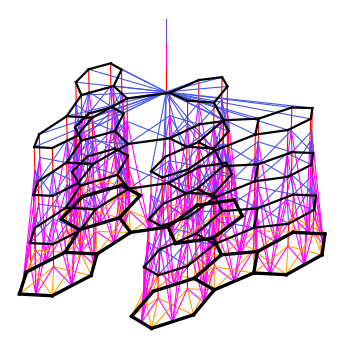
\includegraphics[height=\paperheight]{../paper/figures/3d-nets/net1.png}};\end{tikzpicture}}

\title{Learning Molecular Fingerprints\\from the Graph Up}

\author{
\vspace{-0.5cm}\\
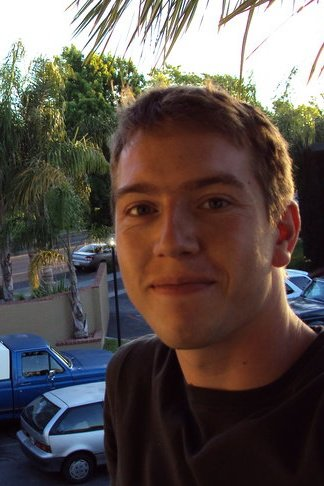
\includegraphics[height=0.16\textwidth, trim=15mm 25mm 0mm 25mm, clip]{talkfigs/david2}
\qquad\qquad
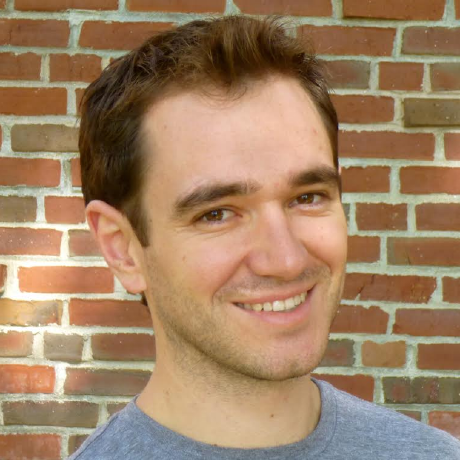
\includegraphics[height=0.16\textwidth]{talkfigs/dougal} \\
David Duvenaud, Dougal Maclaurin, \\
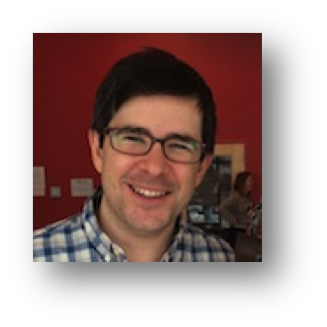
\includegraphics[height=0.16\textwidth, trim=5mm 12mm 12mm 5mm, clip]{talkfigs/jorge}
\qquad\qquad
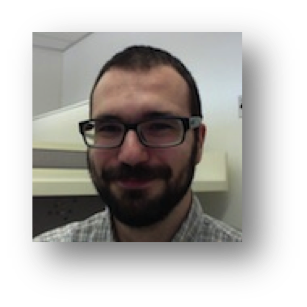
\includegraphics[height=0.16\textwidth, trim=5mm 12mm 12mm 5mm, clip]{talkfigs/rafa}
\qquad\qquad \\
Jorge Aguilera-Iparraguirre, Rafael G\'omez-Bombarelli, \\
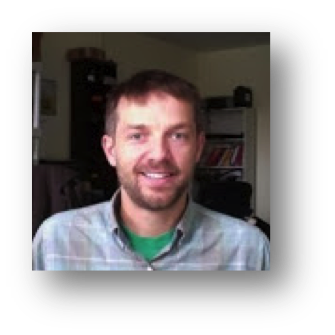
\includegraphics[height=0.16\textwidth, trim=5mm 12mm 12mm 5mm, clip]{talkfigs/tim}
\qquad\qquad
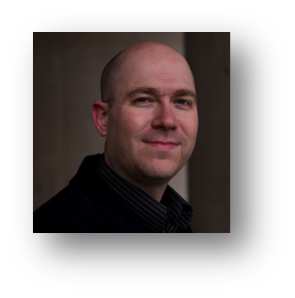
\includegraphics[height=0.16\textwidth, trim=5mm 12mm 12mm 5mm, clip]{talkfigs/alan}
\qquad\qquad
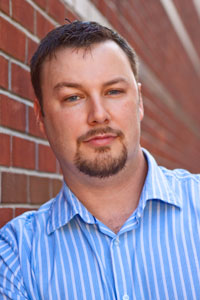
\includegraphics[height=0.16\textwidth]{talkfigs/adams}
\\
Timothy Hirzel, Al\'an Aspuru-Guzik, Ryan P. Adams}

\institute{Harvard University}

\begin{document}

\frame[plain] {\titlepage}
\setbeamertemplate{background canvas}{}

\frame[plain]{\frametitle{Motivation}
\begin{columns}
\hspace{-1cm}\begin{column}{6cm}
\begin{itemize} 
  \item Want to do regression on molecules
  \item For virtual screening of drugs, materials, etc.
  \item Problem: Molecules can be any size and shape
  \item Only know how to learn from fixed-size examples.
  \item How to take a molecule in and produce a fixed-size vector?
\end{itemize}
\end{column}
\begin{column}{5cm}
\hspace{-1cm}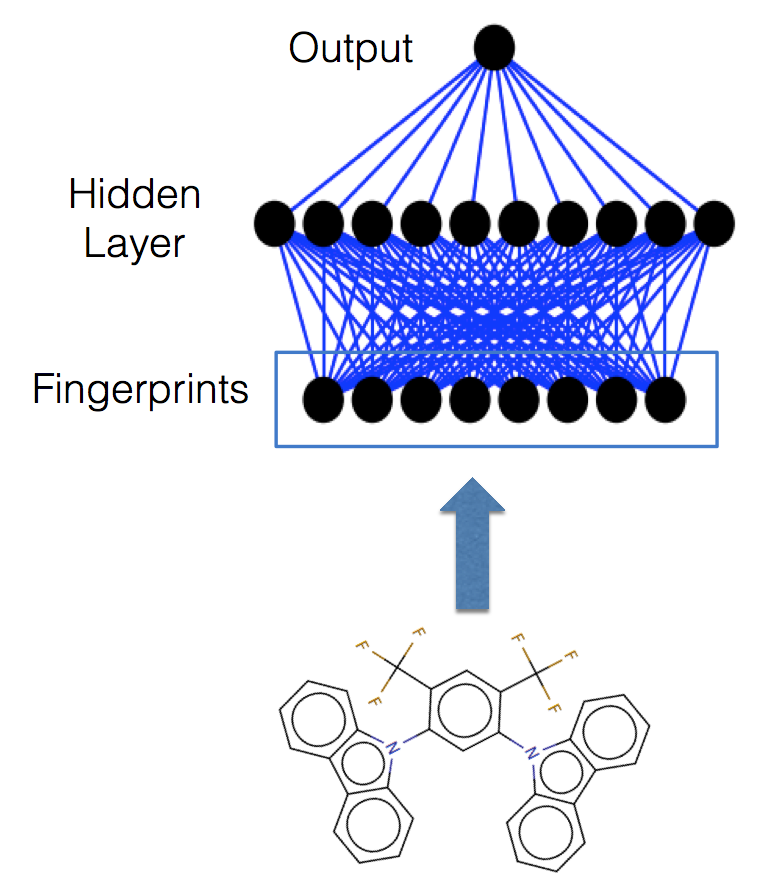
\includegraphics[width=6cm]{talkfigs/how-fingerprints.png}
\end{column}
\end{columns}}

\frame[plain]{\frametitle{Circular Fingeprints}
\begin{columns}
\begin{column}{5.5cm}
\begin{itemize} 
  \item Standard method lists all substructures below a certain size
  \item Can do this by combining hashes of each atom with and bonded neighbors
  \item Hash value indexes into a fixed-sized vector
  \item Problem: can't optimize with gradients
\end{itemize}
\end{column}
\begin{column}{5cm}
\includegraphics[width=6cm]{../../DeepMoleculesData/experiments/2015-06-01-fig1/1/fingerprint_computation_schematic.pdf}
\end{column}
\end{columns}}

\frame[plain]{\frametitle{What would Ryan do?}
\begin{columns}
\begin{column}{5.5cm}
\begin{itemize} 
  \item Maybe we can build a message-passing network
  \item same function is applied to each node (atom) and its neighbors
  \item Like a convolutional net
  \item At the top, add all node's vectors together
  \item If we use a softmax, this generalizes circular fingerprints
\end{itemize}
\end{column}
\begin{column}{5cm}
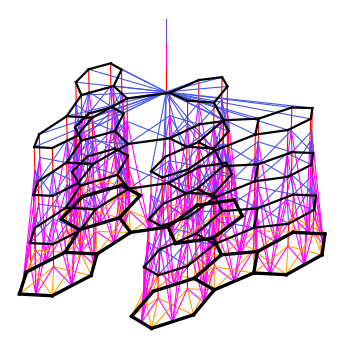
\includegraphics[width=6cm]{../paper/figures/3d-nets/net1.png}
\end{column}
\end{columns}}

\frame[plain]{\frametitle{Continuous-izing Circular Fingerprints}
\hspace{-1cm}\begin{minipage}[t]{0.53\columnwidth}
\begin{algorithm}[H]
\caption*{Circular fingerprints} 
\label{alg:ecfp} 
\scriptsize%
\begin{algorithmic}[1]
\State \textbf{Input:} {molecule, radius $R$, fingerprint length $S$}
\State \textbf{Initialize:} {fingerprint vector $\vf \leftarrow \vzero_S$}
\For {each atom $a$ in molecule} 
    \State $\vr_a \leftarrow g(a)$ \Comment {lookup atom features}
\EndFor
\For {$L = 1$ to $R$} \Comment {for each layer}
	\For {each atom $a$ in molecule}
		\State $\vr_{1} \dots \vr_{N} = \textnormal{neighbors}(a)$
		\State $\vv \leftarrow [\vr_a, \vr_{1}, \dots, \vr_{N}]$ \Comment {concatenate}
		\State $\vr_a \leftarrow \textnormal{hash}(\vv)$ \Comment {hash function}
		\State $i \leftarrow \textnormal{mod}(r_a, S)$ \Comment {convert to index}		
		\State $\vf_{i} \leftarrow 1$ \Comment {Write 1 at index}
	\EndFor
\EndFor
\State \textbf{Return:} {binary vector $\vf$}
\end{algorithmic}
\end{algorithm}
\end{minipage}
\hfill
\begin{minipage}[t]{0.49\columnwidth}
\begin{algorithm}[H]
\caption*{Neural graph fingerprints} 
\label{alg:neural} 
\scriptsize%
\begin{algorithmic}[1]
\State \textbf{Input:} {molecule, radius $R$, {\color{myfavblue} weights $H_1^1 \dots H_R^5$, output weights $W_1 \dots W_R$}}
\State \textbf{Initialize:} {fingerprint vector $\vf \leftarrow \vzero_S$}
\For {each atom $a$ in molecule} 
	\State $\vr_a \leftarrow g(a)$ \Comment {lookup atom features}
\EndFor
\For {$L = 1$ to $R$} \Comment {for each layer}
    \For {each atom $a$ in molecule}
		\State $\vr_{1} \dots \vr_{N} = \textnormal{neighbors}(a)$
		\State $\vv \leftarrow {\color{myfavblue} \vr_a + \sum_{i=1}^{_{N}} \vr_{i}}$ \Comment{{\color{myfavblue}sum}}
		%\State $\vr_a \leftarrow {\color{myfavblue} \vf_{\theta_L}}(v)$ \Comment {{\color{myfavblue} smooth function}}
		\State $\vr_a \leftarrow {\color{myfavblue} \sigma(\vv H_L^N)}$ \Comment{{\color{myfavblue} smooth function}}
		\State $\vi \leftarrow {\color{myfavblue} \textnormal{softmax}(\vr_a W_L)}$ \Comment{{\color{myfavblue} sparsify}}
		\State $\vf \leftarrow {\color{myfavblue} \vf + \vi}$ \Comment{{\color{myfavblue}add to fingerprint}}
    \EndFor
\EndFor
\State \textbf{Return:} { {\color{myfavblue} real-valued} vector $\vf$}
\end{algorithmic}
\end{algorithm}
\end{minipage}

Every non-differentiable operation is replaced with a differentiable analog.
}

\frame[plain]{\frametitle{Generalizing Circular Fingerprints}
\begin{columns}
\hspace{-1cm}\begin{column}{6cm}
\begin{itemize} 
  \item If we generalize existing fingerprints, we can't not win (unless we overfit)
  \item large random weights makes neural nets act like hash functions
  \only<1>{\item Looked at similarities between pairwise distances.}
  \only<2>{\item Looked at performance of random weights.}
\end{itemize}
\end{column}
\begin{column}{5cm}
\hspace{-1cm}\includegraphics<1>[width=6cm]{../../DeepMoleculesData/experiments/2015-05-04-compare-fingerprints/92-distance/morg_conv_corr.pdf}
\includegraphics<2>[width=6cm]{../../DeepMoleculesData/experiments/2015-05-25-delaney/43-random-vs-depth/figures/all_rmsestest_rmse.pdf}
\end{column}
\end{columns}}

\frame[plain]{\frametitle{Performance}
\begin{columns}
\scriptsize
\begin{tabular}{r|lll}
Dataset                      &   Solubility & Drug efficacy  & Photovoltaic efficiency \\
Units                        &   log Mol/L                            & EC$_{50}$ in nM                        & percent \\
\midrule
Predict mean                 & 4.29 $\pm$ 0.40        & 1.47 $\pm$ 0.07         & 6.40 $\pm$ 0.09 \\
Circular FPs + linear layer  & 1.84 $\pm$ 0.08        & \bf{1.13} $\pm$ 0.03    & 2.62 $\pm$ 0.07 \\
Circular FPs + neural net    & 1.40 $\pm$ 0.15        & 1.24 $\pm$ 0.03         & 2.04 $\pm$ 0.07 \\ 
Neural FPs + linear layer    & 0.74 $\pm$ 0.09        & \bf{1.16} $\pm$ 0.03    & 2.71 $\pm$ 0.13 \\  
Neural FPs + neural net      & \bf{0.53} $\pm$ 0.07   & \bf{1.17} $\pm$ 0.03    & \bf{1.44} $\pm$ 0.11
\end{tabular}
%\label{table:main results}
%\caption{Mean predictive accuracy of neural fingerprints compared to standard circular fingerprints.}
\end{columns}

\vspace{1cm}

\begin{itemize}
%\item Still need to include other benchmarks and baselines
\item Could also try varying depth of neural net on top (used one hidden layer here)
\end{itemize}
}

\frame[plain]{\frametitle{Interpretability}
\begin{columns}
\begin{column}{6cm}
\begin{itemize} 
  \item Circular fingerprints activate for a single substructure
  \item No generalization
  \item No notion of similarity
  \item Let's put a linear layer on top of neural fingerprints and examine which fragments activate most predictive features.
\end{itemize}
\end{column}
\begin{column}{5cm}
\hspace{-1cm}\includegraphics[width=6cm]{../../DeepMoleculesData/experiments/2015-06-01-fig1/1/fingerprint_computation_schematic.pdf}
\end{column}
\end{columns}}


\newcommand{\molfeature}[2]{\includegraphics[width=3cm, clip, trim = 2mm 3mm 2mm 3mm]{../../DeepMoleculesData/experiments/2015-05-30-visualize-fps/1/figures/fp_#1_highlight_#2.pdf}}%

\frame[plain]{\frametitle{Interpretability: Solubility}
Fragments activating feature most predictive of solubility:

\molfeature{15}{0} \molfeature{15}{3} \molfeature{15}{2}

most predictive of insolubility:
\molfeature{18}{4} \molfeature{18}{1} \molfeature{18}{2}
}

\frame[plain]{\frametitle{Interpretability: Toxicity}
Fragments most activated by toxicity feature on SR-MMP dataset:

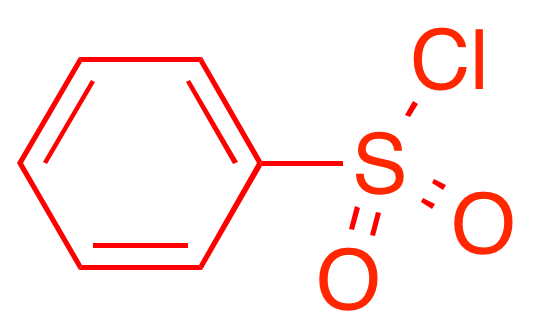
\includegraphics[width=2.2cm]{../paper/figures/jorge-figures/7.png} \qquad
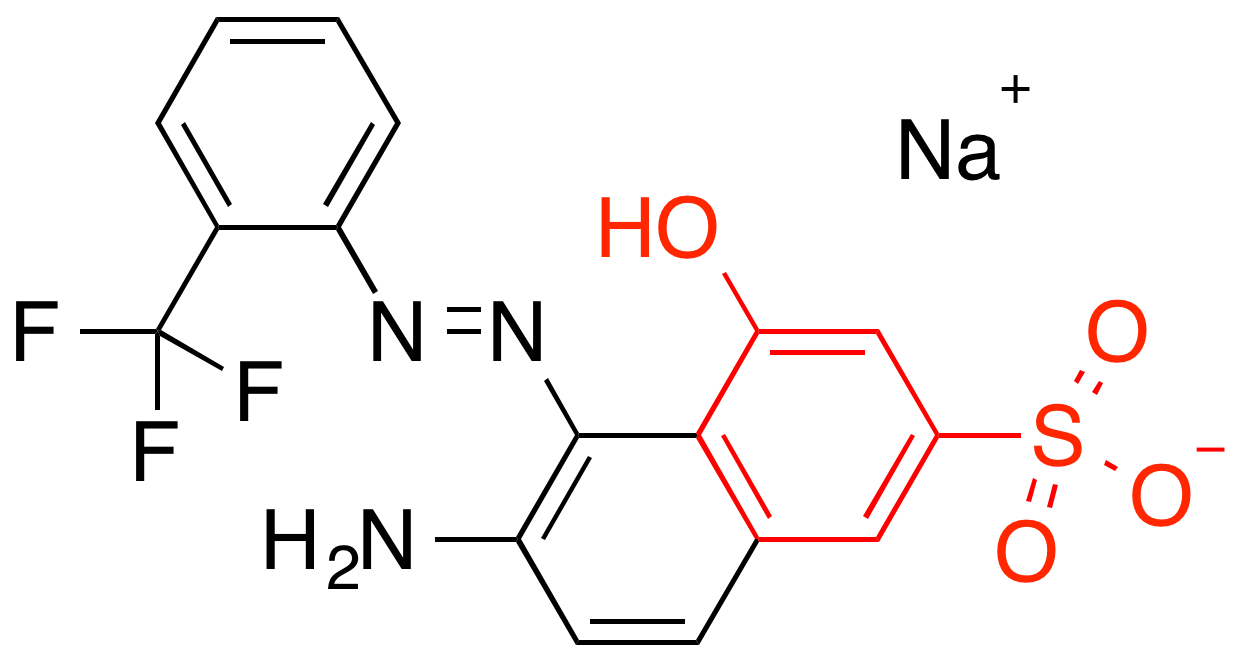
\includegraphics[width=3.3cm]{../paper/figures/jorge-figures/8.png} \qquad
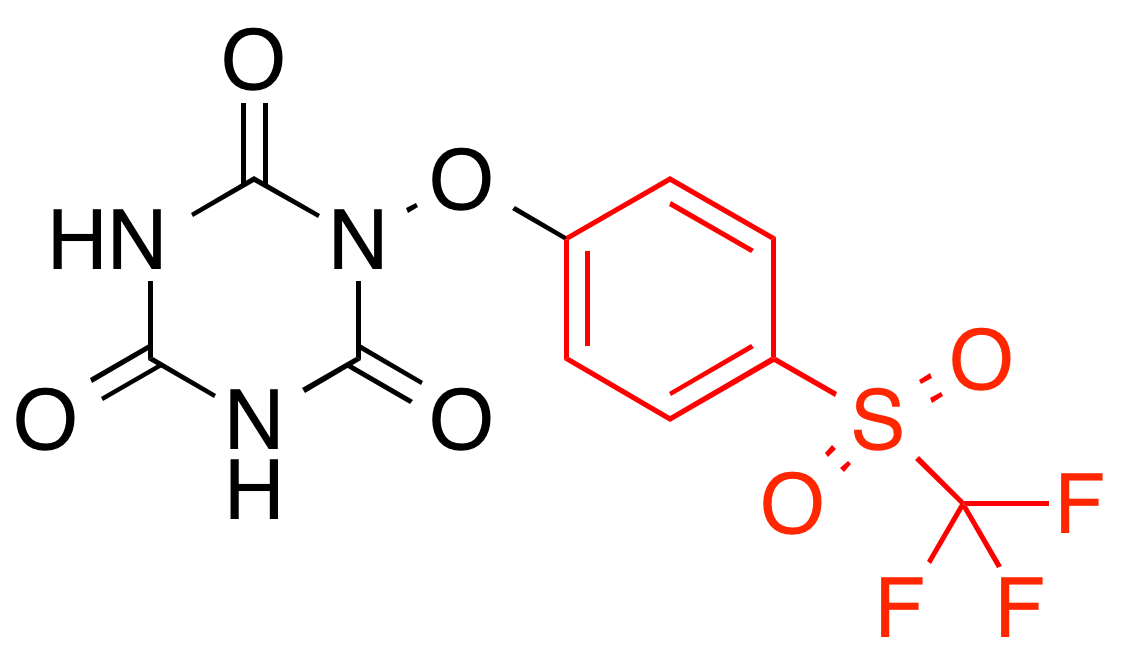
\includegraphics[width=3.3cm]{../paper/figures/jorge-figures/9.png}

Fragments most activated by toxicity feature on NR-AHR dataset:

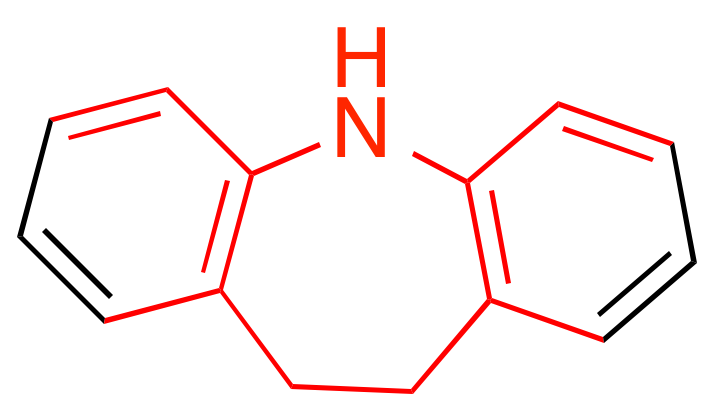
\includegraphics[width=2.2cm]{../paper/figures/jorge-figures/10.png} \qquad
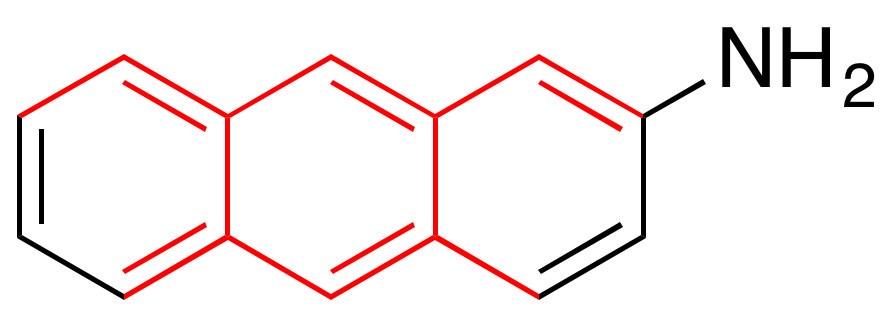
\includegraphics[width=3.3cm]{../paper/figures/jorge-figures/11.png} \qquad
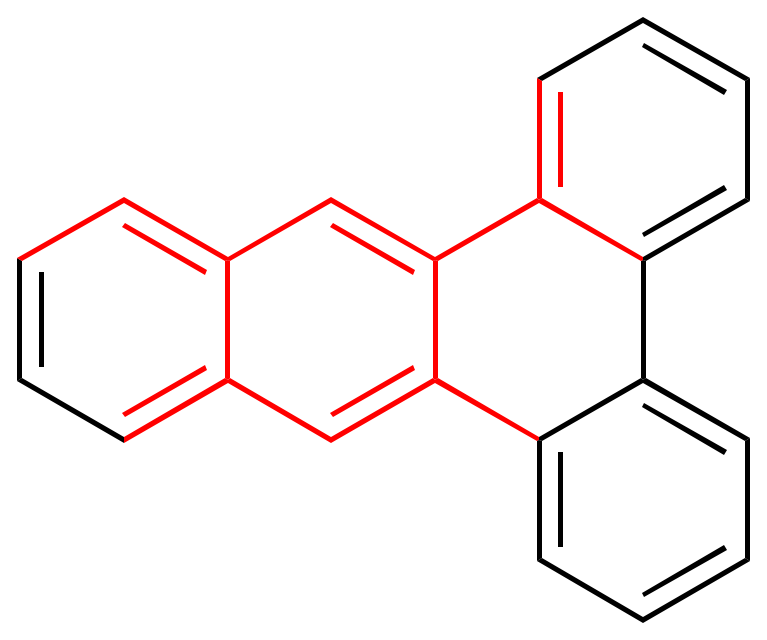
\includegraphics[width=2.9cm]{../paper/figures/jorge-figures/12.png}
}

\frame[plain]{\frametitle{Future Work}
\begin{columns}
\hspace{-1cm}
\begin{column}{6cm}
\begin{itemize} 
  \item Limitation: Slow because of so many weight transforms
  \item Could use low-rank weight matrices
  \item Limitation: All features are local
  \item Could learn to ``parse'' molecules
  \item But how to take gradients?  
\end{itemize}
\end{column}
\begin{column}{5cm}
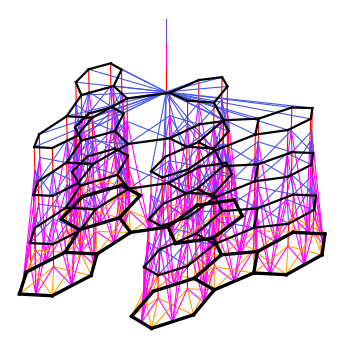
\includegraphics[width=6cm]{../paper/figures/3d-nets/net1.png}
\end{column}
\end{columns}}

\bibliography{../paper/references.bib}
\bibliographystyle{../paper/include/icml2015}
\end{document}
